\title[ASD - Analisi di algoritmi]{\textbf{Algoritmi e Strutture Dati}\\[18pt]Analisi di algoritmi\\Funzioni di costo, notazione asintotica}


%-------------------------------------------------------------------------
\FrameTitle{}

% %-------------------------------------------------------------------------
% \begin{PlainFrame}{Sommario}
%  \tableofcontents
% \end{PlainFrame}

%%%%%%%%%%%%%%%%%%%%%%%%%%%%%%%%%%%%%%%%%%%%%%%%%%%%%%%%%%%%%%%%%%%%%%%%%%
\section{Notazione asintotica}

\subsection{Definizioni}

\begin{frame}{Notazioni $O$, $\Omega$, $\Theta$}

\vspace{-9pt}
\begin{myboxtitle}[Definizione -- Notazione $O$]
Sia $g(n)$ una funzione di costo; indichiamo con $O(g(n))$ l'insieme
delle funzioni $f(n)$ tali per cui:\\[-6pt]
\[
  \exists c>0, \exists m \geq 0: \alert{f(n) \leq cg(n)}, \forall n \geq m
\]
\end{myboxtitle}

\medskip
\begin{itemize}
\item Come si legge: $f(n)$ è “\alert{O grande}” (big-O) di $g(n)$
\item Come si scrive: $f(n) = O(g(n))$
\item $g(n)$ è un \alert{limite asintotico superiore} per $f(n)$
\item $f(n)$ cresce al più come $g(n)$
\end{itemize}

\end{frame}

\begin{frame}{Notazioni $O$, $\Omega$, $\Theta$}

\vspace{-9pt}
\begin{myboxtitle}[Definizione -- Notazione $\Omega$]
Sia $g(n)$ una funzione di costo; indichiamo con $\Omega(g(n))$ l'insieme
delle funzioni $f(n)$ tali per cui:\\[-6pt]
\[
  \exists c>0, \exists m \geq 0: \alert{f(n) \geq cg(n)}, \forall n \geq m
\]
\end{myboxtitle}

\medskip
\begin{itemize}
\item Come si legge: $f(n)$ è “\alert{Omega grande}”  di $g(n)$
\item Come si scrive: $f(n) = \Omega(g(n))$
\item $g(n)$ è un \alert{limite asintotico inferiore} per $f(n)$
\item $f(n)$ cresce almeno quanto $g(n)$
\end{itemize}
\end{frame}

\begin{frame}{Notazioni $O$, $\Omega$, $\Theta$}

\vspace{-9pt}
\begin{myboxtitle}[Definizione -- Notazione $\Theta$]
Sia $g(n)$ una funzione di costo; indichiamo con $\Theta(g(n))$ l'insieme
delle funzioni $f(n)$ tali per cui:\\[-6pt]
\[
  \exists c_1>0, \exists c_2>0, \exists m \geq 0: \alert{c_1g(n) \leq f(n) \leq c_2g(n)}, \forall n \geq m
\]
\end{myboxtitle}

\medskip
\begin{itemize}
\item Come si legge: $f(n)$ è “\alert{Theta}” di $g(n)$
\item Come si scrive: $f(n) = \Theta(g(n))$
\item $f(n)$ cresce esattamente come $g(n)$
\item $f(n) = \Theta(g(n))$ se e solo se $f(n) = O(g(n))$ e $f(n) = \Omega(g(n))$
\end{itemize}

\end{frame}

\begin{frame}{Graficamente}
  
\begin{center}
\vspace{-12pt}
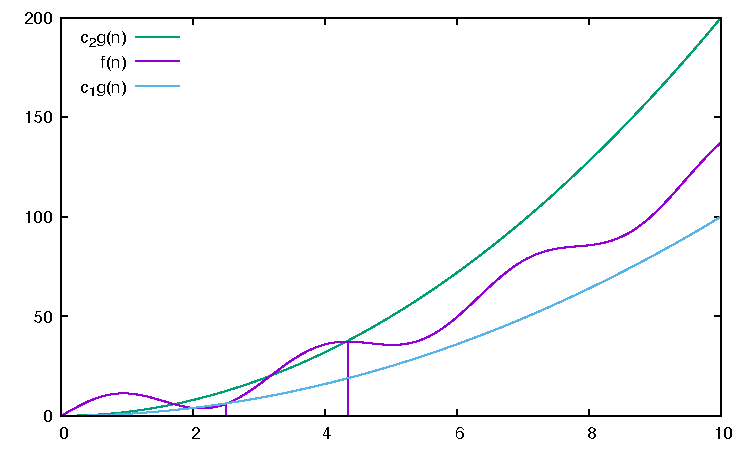
\includegraphics[width=0.9\textwidth]{plot-3.pdf}
\end{center}
  
\end{frame}


\subsection{Esercizi}

\begin{frame}{Vero o falso?}

\begin{exampleblock}{}
\[
  \alert{f(n) = 10 n^3 + 2 n^2 + 7 \stackrel{?}{=} O(n^3)  }
\]
\end{exampleblock}

Dobbiamo provare che $\exists c>0, \exists m \geq 0: f(n) \leq cn^3, \forall n \geq m$

\begin{align*}
f(n) &=    10n^3 +2n^2 + 7 \\
     &\leq 10n^3 +2n^3 + 7 && \forall  n \geq 1\\
     &\leq 10n^3 +2n^3 + 7n^3 && \forall n \geq 1 \\
     &=    19n^3 \\
     &\stackrel{?}{\leq} cn^3
\end{align*}
che è vera per ogni $c \geq 19$ e per ogni $n \geq 1$, quindi $m=1$.
\end{frame}

\begin{frame}{Graficamente}

\begin{center}
\vspace{-12pt}
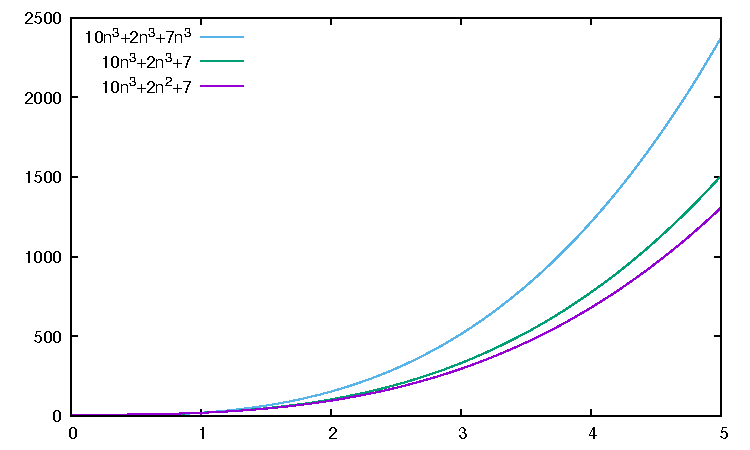
\includegraphics[width=0.9\textwidth]{plot-0.pdf}
\end{center}

\end{frame}

\begin{frame}{Non è l'unico modo di procedere}

\begin{exampleblock}{}
\[
  \alert{f(n) = 10 n^3 + 2 n^2 + 7 \stackrel{?}{=} O(n^3)}
\]
\end{exampleblock}

Dobbiamo provare che $\exists c>0, \exists m \geq 0: f(n) \leq cn^3, \forall n \geq m$

\begin{align*}
f(n) &=    10n^3 +2n^2 + 7 \\
     &\leq 10n^3 +2n^3 + 7 && \forall n \geq 1\\
     &\leq 10n^3 +2n^3 + n^3 && \forall n \geq \sqrt[3]{7}\\
     &=    13n^3 \\
     &\stackrel{?}{\leq} cn^3
\end{align*}
che è vera per ogni $c \geq 13$ e per ogni $n \geq \sqrt[3]{7}$, quindi usiamo $m=2$
\end{frame}

\begin{frame}{Graficamente}

\begin{center}
\vspace{-12pt}
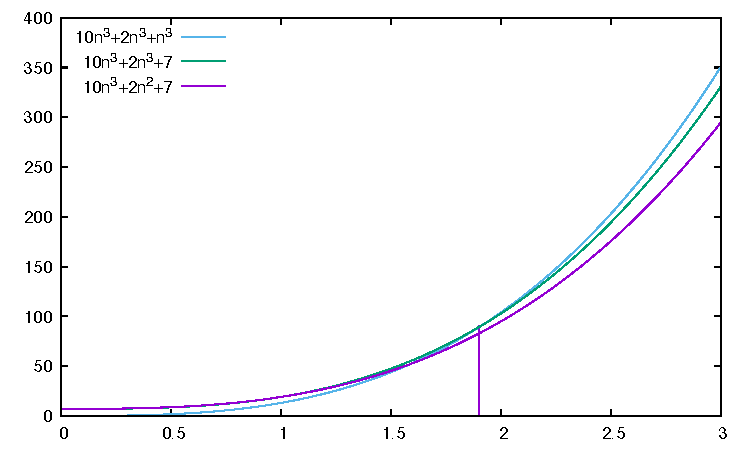
\includegraphics[width=0.9\textwidth]{plot-0bis.pdf}
\end{center}

\end{frame}


\begin{frame}{Vero o falso?}

\begin{exampleblock}{}
\[ 
  \alert{f(n) = 3 n^2 + 7n \stackrel{?}{=} \Theta(n^2)}  
\]
\end{exampleblock}

\begin{overprint}

\onslide<1|handout:0>
\textbf{Limite inferiore}: $\exists c_1>0, \exists m_1 \geq 0: f(n) \geq c_1n^2, \forall n \geq m_1$

\onslide<2|handout:1>
\textbf{Limite inferiore}: $\exists c_1>0, \exists m_1 \geq 0: f(n) \geq c_1n^2, \forall n \geq m_1$

\begin{align*}
f(n) &= 3n^2 + 7n \\
     &\geq 3n^2 && \text{Per $n \geq 0$} \\
     &\stackrel{?}{\geq} c_1n^2
\end{align*}
che è vera per ogni $c_1 \leq 3$ e per ogni $n \geq 0$, quindi $m_1=0$

\onslide<3|handout:0>
\textbf{Limite superiore}: $\exists c_2>0, \exists m_2 \geq 0: f(n) \leq c_2n^2, \forall n \geq m_2$

\onslide<4|handout:2>
\textbf{Limite superiore}: $\exists c_2>0, \exists m_2 \geq 0: f(n) \leq c_2n^2, \forall n \geq m_2$

\begin{align*}
f(n) &=    3n^2 + 7n \\
     &\leq 3n^2 + 7n^2 && \text{Per $n \geq 1$}\\
     &=    10n^2 \\
     &\stackrel{?}{\leq} c_2n^2
\end{align*}
che è vera per ogni $c_2 \geq 10$ e per ogni $n \geq 1$, quindi $m_2=1$

\onslide<5|handout:3>
\textbf{Notazione $\Theta$}: \[
\exists c_1>0, \exists c_2>0, \exists m \geq 0:  c_1 n^2 \leq f(n) \leq c_2n^2, \forall n \geq m
\]
Con questi parametri:
\begin{align*}
c_1 &= 3 \\
c_2 &= 10 \\
m &= \max \{ m_1, m_2 \} = \max \{ 0, 1 \} = 1
\end{align*}

\end{overprint}

\end{frame}

\begin{frame}{Graficamente}

\begin{center}
\vspace{-12pt}
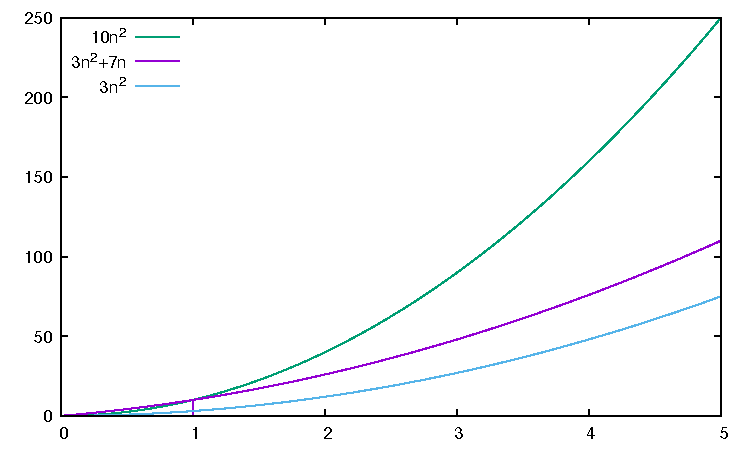
\includegraphics[width=0.9\textwidth]{plot-1.pdf}
\end{center}

\end{frame}

\begin{frame}{Vero o falso?}
  
\begin{exampleblock}{}
\[ 
  \alert{n^2 \stackrel{?}{=} O(n)}
\]
\end{exampleblock}

\bigskip
Dobbiamo dimostrare che $\exists c>0, \exists m>0: n^2 \leq cn, \forall n \geq m$

\begin{itemize}
\item Otteniamo questo: $n^2 \leq cn \Leftrightarrow c \geq n$
\item Questo significa che $c$ cresce con il crescere di $n$, ovvero che non 
possiamo scegliere una costante $c$ 
\end{itemize}

\end{frame}

\begin{frame}{Graficamente}

\begin{center}
\vspace{-12pt}
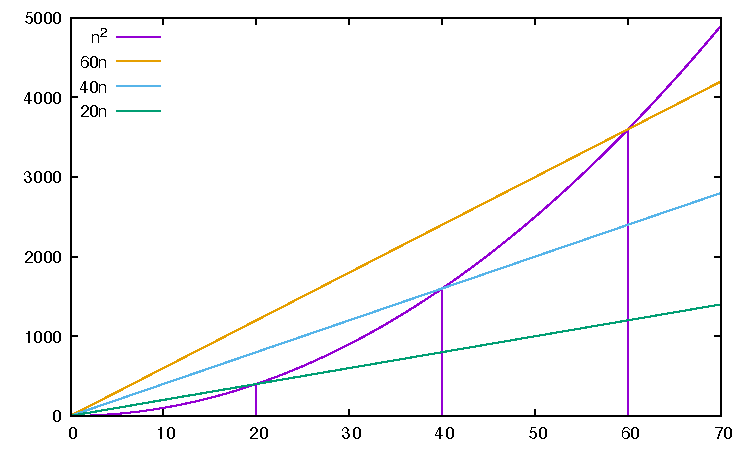
\includegraphics[width=0.9\textwidth]{plot-nvsn2.pdf}
\end{center}

\end{frame}

\begin{frame}{Vero o falso?}

\begin{exampleblock}{}
\[
  \alert{n^2 \stackrel{?}{=} O(n^3)}
\]
\end{exampleblock}

\bigskip
Dobbiamo dimostrare che $\exists c>0, \exists m>0: n^2 \leq cn^3, \forall n \geq m$

\begin{itemize}
\item Otteniamo questo: $n^2 \leq cn^3 \Leftrightarrow c \geq \frac{1}{n}$
\item La funzione $1/n$ è monotona decrescente per $n>0$. 
\item In altre parole, possiamo prendere un qualunque valore $m$ (e.g., $m=1$), e prendere un costante $c \geq 1/m$, come ad esempio $c=1$.
\end{itemize}

\end{frame}






